\documentclass[12pt,a4paper]{article}
\usepackage[UTF8]{ctex}
\usepackage{amsmath}
\usepackage{graphicx}
\usepackage{multirow}
\title{存内计算下的FFT分级计算}
\author{刘润}

\begin{document}

\maketitle
\section{FFT混合基分解}

\subsection{FFT混合基分解一般形式}
对于$N$点$DFT$,如果$N$是一个复合数,它可以分解成一些因子的乘积,则可以用$FTT$的一般算法,即混合基$FFT$算法,
而基-2算法只是这种一般算法的特例。

若$N$可以表示为复合数$N=r_1r_2 \cdots r_L$,则对于$n<r_1r_2 \cdots r_L$,的任何一个正整数$n$,可以按照
$L$基$r_1$,$r_2$,$\cdots$,$r_L$ 表示为多基多进制形式$(n_{L-1}n_{L-2} \cdots n_1n_0)_{r_1r_2 \cdots r_L}$,
这一多基多进制所代表的数值为:
\begin{equation}
    (n)_{10} = n_{L-1}(r_2r_3 \cdots r_L) + n_{L-2}(r_3r_4 \cdots r_L) + \cdots + n_1n_L + n_0
\end{equation}
其倒位序形式为$[\rho(n)]_{r_Lr_{L-1} \cdots r_2r_1} = (n_0n_1 \cdots n_{L-2}n_{L-1})_{r_Lr_{L-1} \cdots r_2r_1}$,它所代表的数值为:
\begin{equation}
    [\rho(n)]_{10}=n_0(r_1r_2 \cdots r_{L-1}) + n_1(r_1r_2 \cdots r_{L-2}) + \cdots + n_{L-2}r_1 + n_{L-1}
\end{equation}
在这一多基多进制的表示中
\begin{equation}
\begin{aligned}
    &n_0 = 0,1,\cdots ,r_{L}-1 \\
    &n_1 = 0,1,\cdots ,r_{L-1}-1 \\
    &\cdots \\
    &n_{L-1} = 0,1,\cdots ,r_1-1
\end{aligned}
\end{equation}


\subsection{512点FFT示例}
下面以512点FFT作为示例讲解,将512点FFT分解为$16*16*2$三级,即$N=16*16*2$,则$r_1=16$,$r_2=16$,$r_3=2$,$L=3$,
则有:

\begin{equation}
    n = n_2(r_2r_3) + n_1r_3 + n_0 = 32n_2 + 2n_1 + n_0
\end{equation}
\begin{equation}
    k = k_0(r_1r_2) + k_1r_1 + k_2 = 256k_0 + 16k_1 + k_2
\end{equation}
\begin{equation}
\begin{aligned}
  n_0,k_0 &: 0 \sim 1 (r_3) \\
  n_1,k_1 &: 0 \sim 15 (r_2) \\
  n_2,k_2 &: 0 \sim 15 (r_1)
\end{aligned}
\end{equation}
所以根据$DFT$公式$X(k) = \sum\limits_{n=0}^{511}x(n)W_{512}^{nk}$,则将公式$(4)\sim (6)$带入可得:
\begin{equation}
\begin{aligned}
    X(k) &= \sum_{n=0}^{511}x(n)W_{512}^{nk} \\
         &= \sum_{n_0=0}^{1} \sum_{n_1=0}^{15} \sum_{n_2=0}^{15} x(n_2,n_1,n_0)
            W_{512}^{(32n_2+2n_1+n_0)(256k_0+16k_1+k_2)} \\
\end{aligned}
\end{equation}
可以得到
\begin{equation}
\begin{aligned}
    X(k) = \sum_{n_0=0}^{1} \sum_{n_1=0}^{15} \sum_{n_2=0}^{15} x(n_2,n_1,n_0)
            &W_{512}^{8192n_2k_0} W_{512}^{512n_2k_1} W_{512}^{32n_2k_2} \\
            &W_{512}^{512n_1k_0} W_{512}^{32n_1k_1} W_{512}^{2n_1k_2}\\
            &W_{512}^{256n_0k_0} W_{512}^{16n_0k_1} W_{512}^{n_0k_2} \\
\end{aligned}
\end{equation}
\begin{equation}
\begin{aligned}
    X(k) &= \sum_{n_0=0}^{1} \sum_{n_1=0}^{15} \sum_{n_2=0}^{15} x(n_2,n_1,n_0)
            W_{512}^{32n_2k_2} W_{512}^{32n_1k_1} W_{512}^{2n_1k_2}
            W_{512}^{256n_0k_0} W_{512}^{16n_0k_1} W_{512}^{n_0k_2} \\
         &= \sum_{n_0=0}^{1} \sum_{n_1=0}^{15} [\sum_{n_2=0}^{15} x(n_2,n_1,n_0)W_{16}^{n_2k_2}]
            W_{512}^{32n_1k_1} W_{512}^{2n_1k_2} W_{512}^{256n_0k_0} W_{512}^{16n_0k_1} W_{512}^{n_0k_2} \\
         &= \sum_{n_0=0}^{1} \sum_{n_1=0}^{15} [X_1(k_2,n_1,n_0) W_{512}^{(2n_1 + n_0)k_2}]
            W_{512}^{32n_1k_1} W_{512}^{16n_0k_1} W_{512}^{256n_0k_0} \\
         &= \sum_{n_0=0}^{1} [\sum_{n_1=0}^{15} X_1^{'}(k_2,n_1,n_0) W_{16}^{n_1k_1}]
            W_{512}^{16n_0k_1} W_{512}^{256n_0k_0} \\
         &= \sum_{n_0=0}^{1} [X_2(k_2,k_1,n_0) W_{512}^{16n_0k_1}]
            W_{512}^{256n_0k_0} \\
         &= \sum_{n_0=0}^{1} X_2^{'}(k_2,k_1,n_0) W_{2}^{n_0k_0} \\
         &= X(k_2,k_1,k_0)
\end{aligned}
\end{equation}
并且有
\begin{equation}
\begin{aligned}
    X_1(k_2,n_1,n_0) &= \sum_{n_2=0}^{15} x(n_2,n_1,n_0)W_{16}^{n_2k_2} \\
    X_1^{'}(k_2,n_1,n_0) &= X_1(k_2,n_1,n_0) W_{512}^{(2n_1 + n_0)k_2}
\end{aligned}
\end{equation}
\begin{equation}
\begin{aligned}
    X_2(k_2,k_1,n_0) &= \sum_{n_1=0}^{15} X_1^{'}(k_2,n_1,n_0) W_{16}^{n_1k_1} \\
    X_2^{'}(k_2,k_1,n_0) &= X_2(k_2,k_1,n_0) W_{512}^{16n_0k_1}
\end{aligned}
\end{equation}
\begin{equation}
    X(k_2,k_1,k_0) = \sum_{n_0=0}^{1} X_2^{'}(k_2,k_1,n_0) W_{2}^{n_0k_0}
\end{equation}
可以很明显看出,512点的FFT可以拆解为16*16*2的三级FFT的级联,公式(10)为第1级16点FFT,公式(11)为第2级16点FFT,
公式(12)为第3级2点FFT。

\section{计算过程}
\subsection{理论计算流程}
根据以上公式,可以得出结论,512点FFT计算可以分解为三级较小规模的FFT计算,并且通过公式$(4) \sim (6)$可以得知
原始信号的输入次序和计算得到信号的输出次序。原始信号为$x(0), x(1), x(2), ..., x(511), x(512)$,输入时读入
的次序为$n=32n_2+2n_1+n_0$。

\begin{figure}[h]
\centering
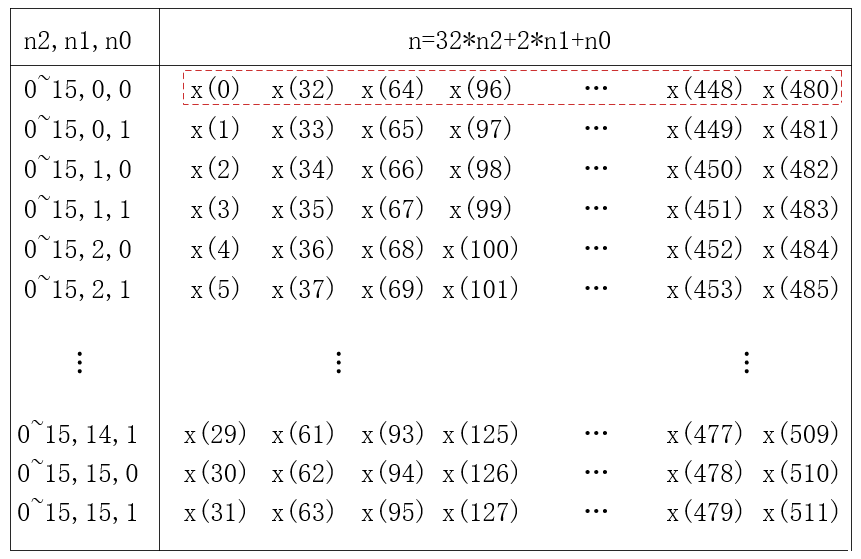
\includegraphics[scale=0.6]{figures/figure1}
\caption{第一级FFT16输入次序}
\end{figure}
原始信号以行为单位并行输入16个数据,作为第一级FFT计算。根据式(10)可以得知,第一级FFT16个数据并行输入,和存储在
FLASH模块中的旋转因子相乘,经过ADC采样之后,得到$X_1$,再与$W_{512}^{(2n_1+n_0)k_2}$相乘完成第一级FFT。所以对于一个
FFT16计算模块来说,以第一行数据为例,其矩阵运算模式为:

\begin{equation}
\begin{bmatrix}
X_1(0) \\ X_1(32) \\ \vdots \\ X_1(480)
\end{bmatrix}
\begin{bmatrix}
W_{16}^0 & W_{16}^0 & W_{16}^0 &... &W_{16}^0 \\
W_{16}^0 & W_{16}^{1\times 1} & W_{16}^{1\times 2} &... &W_{16}^{1\times15} \\
\vdots &\vdots &\vdots &  &\vdots \\
W_{16}^0 & W_{16}^{15\times 1} & W_{16}^{15\times 2} &... &W_{16}^{15\times 15} \\
\end{bmatrix}
\begin{bmatrix}
x(0) \\ x(32) \\ \vdots \\ x(480)
\end{bmatrix}
\end{equation}

\noindent 再将得到的$X_1$向量与$W_{512}^{(2n_1+n_0)k_2}$向量元素对应相乘即可。
\begin{equation}
\begin{bmatrix}
X_1(0) \\ X_1(32) \\ \vdots \\ X_1(480)
\end{bmatrix}
*
\begin{bmatrix}
W_{512}^{(2*0+0)*0} \\ W_{512}^{(2*0+0)*1} \\ \vdots \\ W_{512}^{(2*0+0)*15}
\end{bmatrix}
\rightarrow
\begin{bmatrix}
X_1^{'}(0) \\ X_1^{'}(32) \\ \vdots \\ X_1^{'}(480)
\end{bmatrix}
\end{equation}

重复以上过程,完成第一级FFT16计算。完成之后可以进行第二级FFT16计算,还是按照$n=32n_2+2n_1+n_0$公式,
只不过此时信号输入数据为第一级FFT16计算得到结果,并且次序按照$n_1$进行。将红框内的数据并行输入,进行
第二级FFT16的计算。

\begin{figure}[h]
\centering
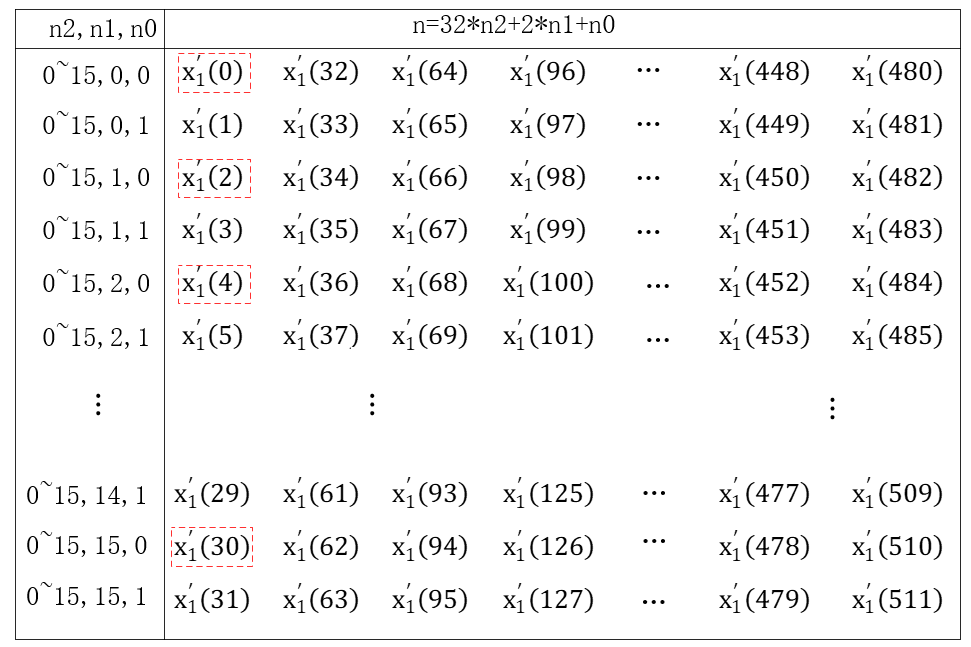
\includegraphics[scale=0.6]{figures/figure2}
\caption{第二级FFT16输入次序}
\end{figure}

\begin{equation}
\begin{bmatrix}
X_2(0) \\ X_2(2) \\ \vdots \\ X_2(30)
\end{bmatrix}
\begin{bmatrix}
W_{16}^0 & W_{16}^0 & W_{16}^0 &... &W_{16}^0 \\
W_{16}^0 & W_{16}^{1\times 1} & W_{16}^{1\times 2} &... &W_{16}^{1\times15} \\
\vdots &\vdots &\vdots &  &\vdots \\
W_{16}^0 & W_{16}^{15\times 1} & W_{16}^{15\times 2} &... &W_{16}^{15\times 15} \\
\end{bmatrix}
\begin{bmatrix}
X_1^{'}(0) \\ X_1^{'}(2) \\ \vdots \\ X_1^{'}(30)
\end{bmatrix}
\end{equation}

\begin{equation}
\begin{bmatrix}
X_2(0) \\ X_2(2) \\ \vdots \\ X_2(30)
\end{bmatrix}
*
\begin{bmatrix}
W_{512}^{16*0*0} \\ W_{512}^{16*0*1} \\ \vdots \\ W_{512}^{16*0*15}
\end{bmatrix}
\rightarrow
\begin{bmatrix}
X_2^{'}(0) \\ X_2^{'}(2) \\ \vdots \\ X_2^{'}(30)
\end{bmatrix}
\end{equation}
\noindent 重复以上过程,可以完成第二级FFT16的计算

\subsection{FFT16的存内计算方法}
存内计算模式对于矩阵乘加计算比较友好,适合FFT这样的矩阵乘法运算。任然以第一级FFT16为例,其第一行原始信号数据输入
后与旋转因子矩阵第一行元素对应相乘相加,得到第一个FFT16计算结果$X_1(0)$,其过程在FLASH块中的计算过程为下图所示。

\begin{figure}[h]
\centering
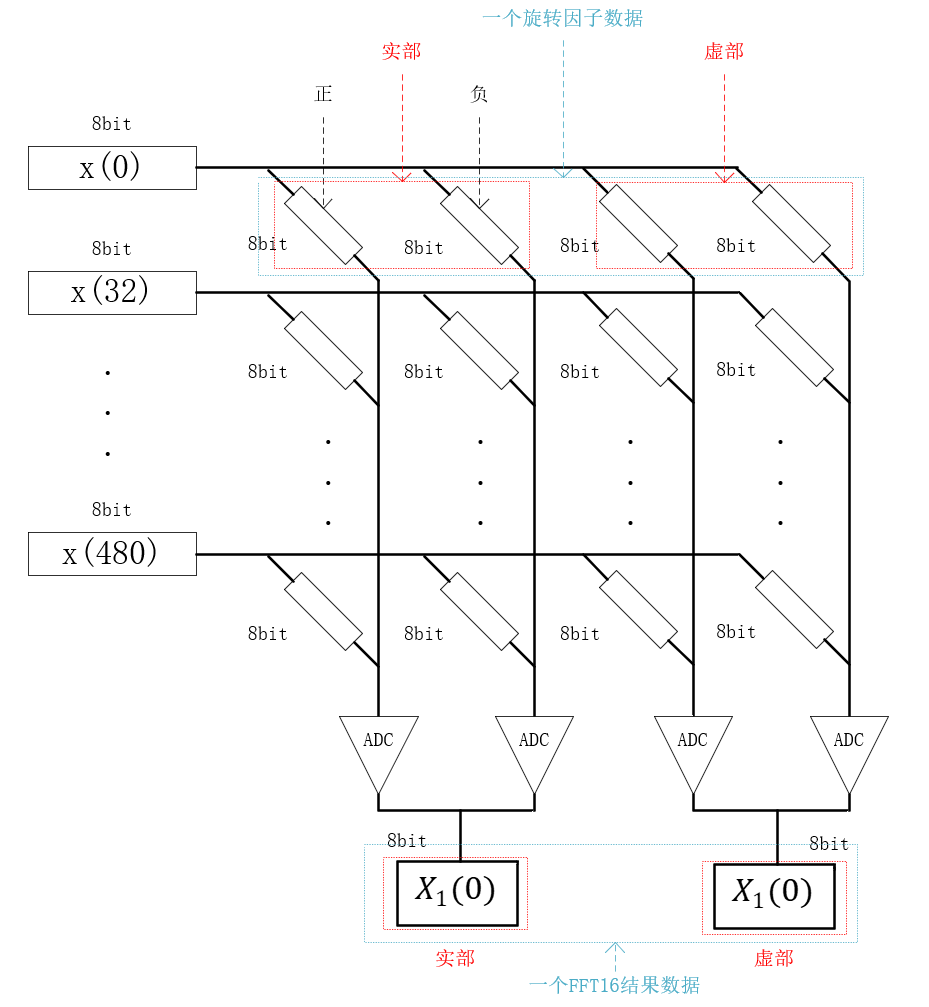
\includegraphics[scale=0.5]{figures/figure3}
\caption{一个FFT16数据在CIM中计算示意图}
\end{figure}

\noindent 则对于一个完整的FFT16模块来说,其在CIM中的计算过程可以如下图所示。
\begin{figure}[h]
\centering
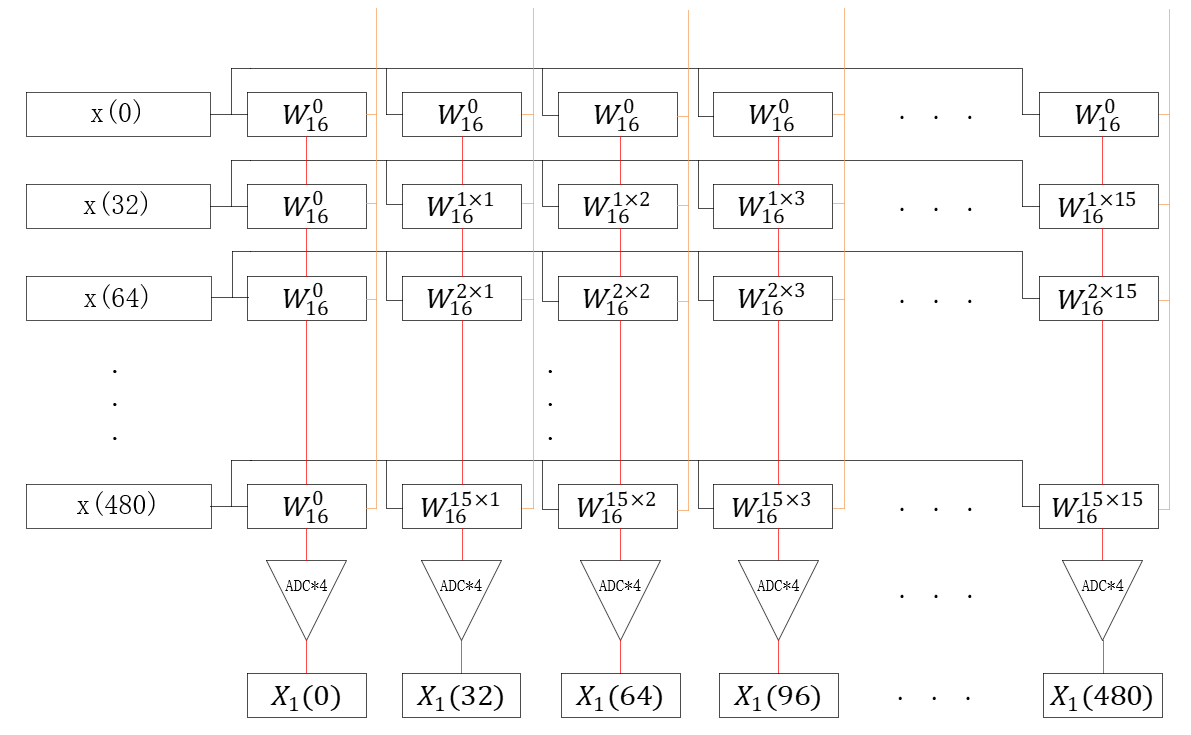
\includegraphics[scale=0.5]{figures/figure4}
\caption{一个FFT16模块在CIM中计算示意图}
\end{figure}

\noindent 所以当有多个FFT16模块在FLASH Core中存在时,其结构图如下图所示。其中存储1中存储的是需要进行FFT计算的
原始数据和在分级计算中产生的中间数据。从存储1模块中每次并行输出16个数据送入到一个FFT16模块中进行计算,在FLASH Core
中完成计算之后并行输出16个模拟结果经过ADC进行转换成为数字结果。随后存储2中根据公式(10)(11)(12)所产生的旋转因子和
FLASH core中产生的数字结果进行相乘,得到第一级的输出结果并且回存到存储1中,这样就完成了第一级FFT16的计算。在下图中
的乘法器矩阵就是为了和旋转因子相乘而设置的。
\begin{figure}[h]
\centering

\includegraphics[scale=0.45]{figures/figure5}
\caption{多个FFT16模块在CIM中计算示意图}
\end{figure}

由此,我们也可以得到一级FFT16的时序输出。
\begin{figure}[h]
\centering
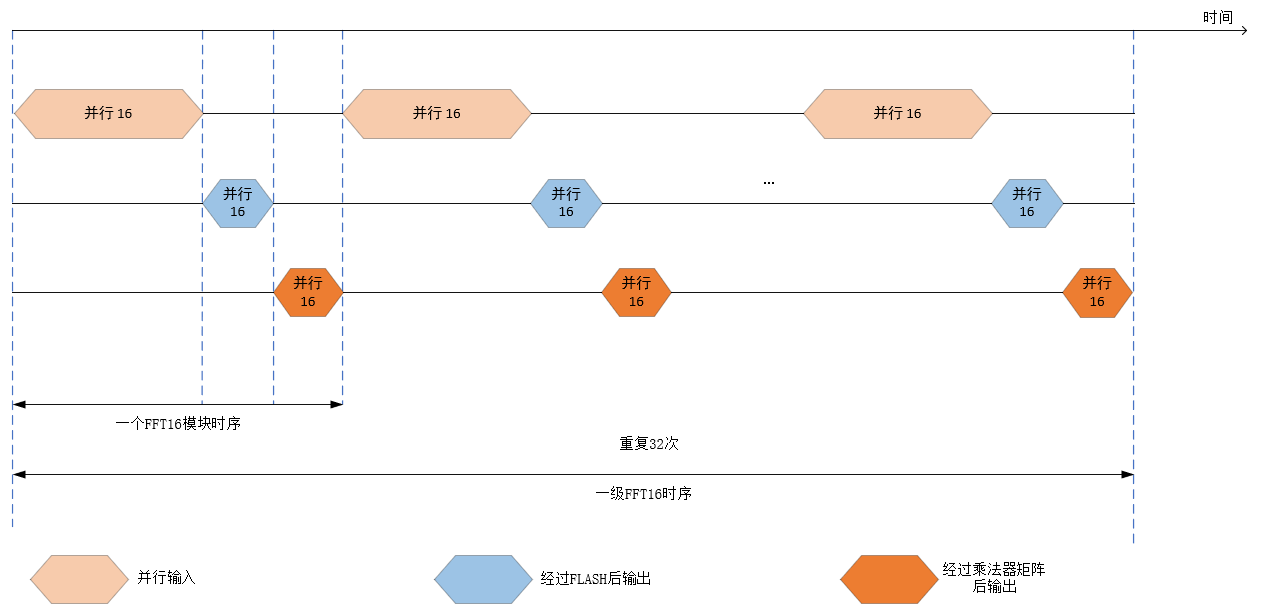
\includegraphics[scale=0.6]{figures/figure6}
\caption{一级FFT16计算时序示意图}
\end{figure}
\noindent 当我们重复上述时序之后,就会得到第二级FFT16时序,从而得到在CIM中FFT计算的完整时序。这是什么东西。这是什么鬼



\begin{table}[htbp]
\centering
\caption{title}
\label{tab1}
    \begin{tabular}{cccccc}
        \hline
        Specification &Proposed &[1](F) &[2](P) &[2]      &[3] \\
        \hline
        FFT Size(N)   &512      &1024   &1024   &1024     &4096   \\
        Technology    &45nm     &65nm   &65nm   &65nm     &65nm   \\
        Vdd           &1V       &0.45V  &0.45V  &0.6V     &1.2V   \\
        Word-length   &8-bit    &12-bit &12-bit &32-bit*  &14-bit  \\
        Power(mW)     &21.66    &12     &123    &60.3     &68.6    \\
        \hline
    \end{tabular}
\end{table}
\end{document} 